\documentclass[compress]{beamer}
\usepackage{ifthen,verbatim}

\newcommand{\isnote}{}
\xdefinecolor{lightyellow}{rgb}{1.,1.,0.25}
\xdefinecolor{darkblue}{rgb}{0.1,0.1,0.7}

%% Uncomment this to get annotations
%% \def\notes{\addtocounter{page}{-1}
%%            \renewcommand{\isnote}{*}
%% 	   \beamertemplateshadingbackground{lightyellow}{white}
%%            \begin{frame}
%%            \frametitle{Notes for the previous page (page \insertpagenumber)}
%%            \itemize}
%% \def\endnotes{\enditemize
%% 	      \end{frame}
%%               \beamertemplateshadingbackground{white}{white}
%%               \renewcommand{\isnote}{}}

%% Uncomment this to not get annotations
\def\notes{\comment}
\def\endnotes{\endcomment}

\setbeamertemplate{navigation symbols}{}
\setbeamertemplate{headline}{\mbox{ } \hfill
\begin{minipage}{5.5 cm}
\vspace{-0.75 cm} \small
\end{minipage} \hfill
\begin{minipage}{4.5 cm}
\vspace{-0.75 cm} \small
\begin{flushright}
\ifthenelse{\equal{\insertpagenumber}{1}}{}{Jim Pivarski \hspace{0.2 cm} \insertpagenumber\isnote/\pageref{numpages}}
\end{flushright}
\end{minipage}\mbox{\hspace{0.2 cm}}\includegraphics[height=1 cm]{../cmslogo} \hspace{0.1 cm} \includegraphics[height=1 cm]{../tamulogo} \hspace{0.01 cm} \vspace{-1.05 cm}}

\newcommand{\s}[1]{{\mbox{\scriptsize #1}}}

\begin{document}
\begin{frame}
\vfill
\begin{center}
\textcolor{darkblue}{\Large Resolving twist: summary and more diagnostic ideas}

\vfill
\begin{columns}
\column{0.3\linewidth}
\begin{center}
\large
Jim Pivarski
\end{center}
\end{columns}

\begin{columns}
\column{0.3\linewidth}
\begin{center}
\scriptsize
{\it Texas A\&M University}
\end{center}
\end{columns}

\vfill
22 October, 2010

\end{center}
\end{frame}

%% \begin{notes}
%% \item This is the annotated version of my talk.
%% \item If you want the version that I am presenting, download the one
%% labeled ``slides'' on Indico (or just ignore these yellow pages).
%% \item The annotated version is provided for extra detail and a written
%% record of comments that I intend to make orally.
%% \item Yellow notes refer to the content on the {\it previous} page.
%% \item All other slides are identical for the two versions.
%% \end{notes}

\small

\begin{frame}
\frametitle{The situation}
\begin{itemize}
\item The discrepancy between the barrel hardware geometry and tracks remains unresolved
\item This means that our ``probability distribution'' for the correct geometry is bimodal: a peak around the track-based result and a peak around the hardware result
\item This is not a usable probability distribution for physics analyses
\item Using the wrong geometry yields a 40\% smearing of a 1.1~TeV/$c^2$ $Z'$ peak: so the ``probability distribution'' is too wide as well as having an unusable shape
\item If this is not resolved, then high-$p_T$ muon analyses will have to be based on tracker-tracks only: worse statistical uncertainty, better-understood systematics
\begin{itemize}
\item that is, all muon alignment work will be ignored
\end{itemize}
\item The deadline for having a firm conclusion about which twist properly represents the real muon system is Nov 5
\end{itemize}
\end{frame}

\begin{frame}
\frametitle{Attempts to resolve it}
\begin{itemize}
\item Comparison with inclinometers: independent measurements say that ends of MABs are not rotated around the beamline
\item Link doesn't see a rotation of the two sides, either, but the ME$-$ side measurement has only one laser
\item HW-barrel 0~T alignment agrees with photogrammetry within wheels, but the PG positions of the wheels have mm-scale uncertainties
\item Track/HW discrepancy does not grow with distance from the beamline (confirmed at residuals level)
\item Endcap $\to$ transfer lines $\to$ barrel provides closure tests, but may not be ready in time
\item New idea: try alignment in ``two-bin mode'' to cancel B-field
\item New idea: look for mismatch with vertical StandAlone cosmics
\end{itemize}
\end{frame}

\begin{frame}
\frametitle{Magnetic field}
\begin{itemize}
\item Might be $B_r$ error instead of the usual $B_z$?  No, I tried some simulations: $B_r$ also makes deviations that grow with distance from the tracker, even with $B_r$ effect partly cancelling $B_z$
\item (Un)lucky cancellation?  Conceivable\ldots
\end{itemize}

\begin{center}
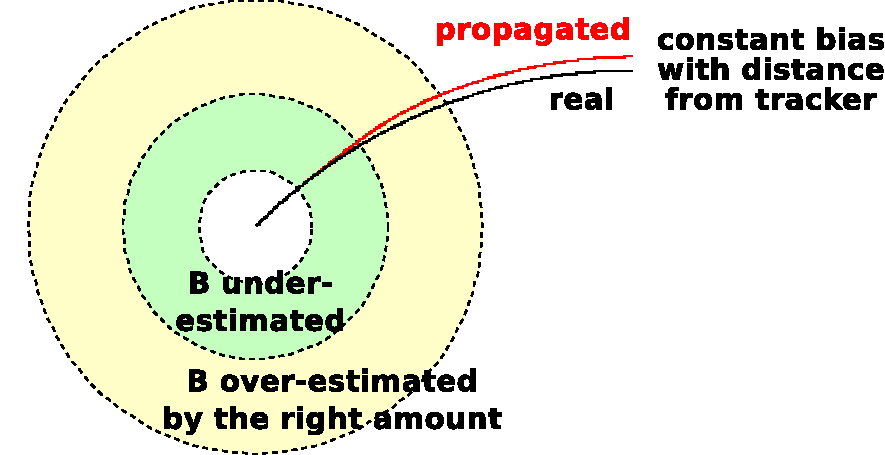
\includegraphics[width=0.8\linewidth]{bfield_hypothesis.pdf}
\end{center}

\begin{itemize}
\item ``Two-bin mode'': compute alignment 1 with $\mu^+$, alignment 2
  with $\mu^-$, align to average and plot differences: cancels sensitivity to $\vec{B}$
 \end{itemize}
\end{frame}

\begin{frame}
\frametitle{Mismatch in vertical cosmics}
\begin{columns}
\column{0.4\linewidth}
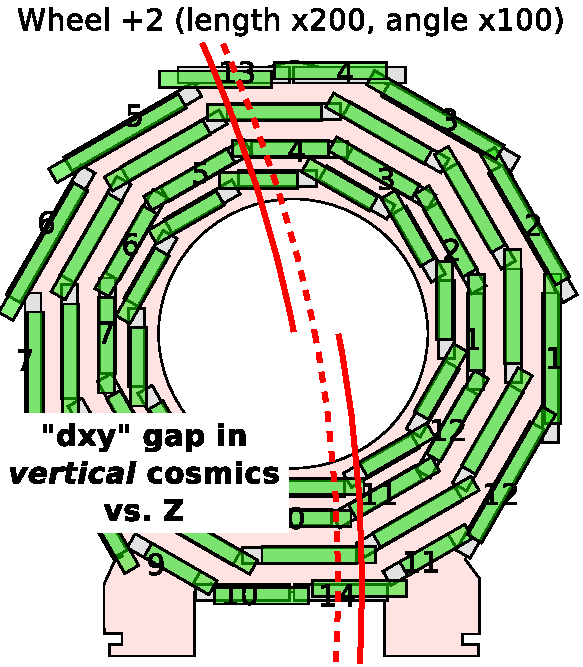
\includegraphics[width=\linewidth]{twist.pdf}

\vspace{0.5 cm}
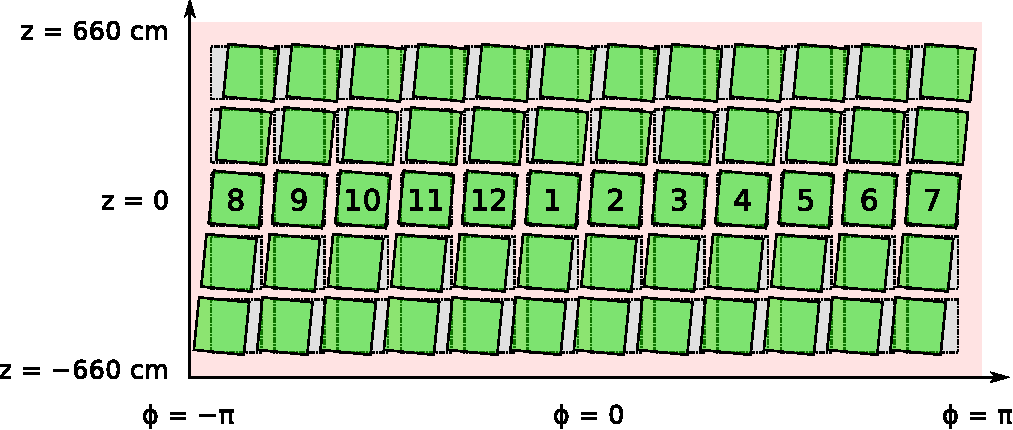
\includegraphics[width=\linewidth]{twist_station.pdf}

\column{0.6\linewidth}
\begin{itemize}
\item At one extreme end of the barrel, twist moves top chambers to
  the left and bottom to the right (they do {\it not} rotate around
  the beamline: that's not {\it our} twist)
\item This would break vertical StandAlone cosmics: $d_{xy}$ gap that
  is proportional to $z$
\item Independent of tracker-to-muon alignment
\item The verticalness of the tracks is crucial: must be
  non-tracker-pointing cosmic rays (StandAloneMuons)
\end{itemize}
\end{columns}
\end{frame}

%% \begin{frame}
%% \frametitle{Outline}
%% \begin{itemize}\setlength{\itemsep}{0.75 cm}
%% \item 
%% \end{itemize}
%% %% \hspace{-0.83 cm} \textcolor{darkblue}{\Large Outline2}
%% \end{frame}

%% \section*{First section}
%% \begin{frame}
%% \begin{center}
%% \Huge \textcolor{blue}{First section}
%% \end{center}
%% \end{frame}

\begin{frame}
\frametitle{The end of this talk}
\begin{itemize}
\item This week, I tried the vertical-track test in MC collisions with
  a twisted geometry--- and learned why non-tracker-pointing is
  essential (it's a 3-D effect)
\begin{itemize}
\item collisions won't work: need straight-down cosmic rays
\item skimming a sample now
\end{itemize}

\item Magnetic field can be easily cancelled by the ``two-bin mode''
  of the alignment algorithm (demonstrated in Feb 2009 when the
  B-field errors were large)
\begin{itemize}
\item for B-field components in any direction (axial, radial, or
  azimuthal), the effect on trajectory depends on the charge of the
  muon: $\vec{B}$ must yield differences between $\mu^+$ and $\mu^-$
\item work on this has started\ldots
\end{itemize}

\item I will be unavailable for next Friday's meeting: results by HyperNews

\item Any other ideas that can lead to a firm conclusion about this
  degree of freedom are encouraged\ldots
\end{itemize}
\label{numpages}
\end{frame}

\end{document}
